\documentclass[9pt]{beamer}
\usepackage{graphicx}
\graphicspath{{Images/}}
\usepackage{media9}
\addmediapath{Videos/}
\usepackage{caption}
\usepackage{multicol}
\usepackage{media9}
\usepackage{xcolor,colortbl}
%\definecolor{green}{rgb}{0.1,0.1,0.1}
\newcommand{\done}{\cellcolor{green}}  %{0.9}
\newcommand{\hcyan}[1]{{\color{green} #1}}
\usepackage{amsmath}
\mode<presentation> {
\usetheme{Warsaw}
}

\usepackage{graphicx} % Allows including images
\usepackage{booktabs} %

\title[Statistical Model for Improved Surface Detection]{A Statistical Model for Improved Surface Detection} % The short title appears at the bottom of every slide, the full title is only on the title page

\author{Samuel Smith} % Your name
\institute[Birmingham City University] % Your institution as it will appear on the bottom of every slide, may be shorthand to save space
{
Birmingham City University \\ % Your institution for the title page
\medskip
\textit{samuel.smith@mail.bcu.ac.uk} % Your email address
}
\date{\today} % Date, can be changed to a custom date

\begin{document}
%--------------------------------------------------------
\begin{frame}
	\titlepage % Print the title page as the first slide
\end{frame}
%--------------------------------------------------------
\section{Problem Definition}
\subsection{Rationale}
%--------------------------------------------------------
\begin{frame}
	\frametitle{Rationale}
		\begin{itemize}
			\item Three dimensional image data is becoming the common modality for many non-destructive testing, image analysis, visualisation and biomedical imaging systems. Typically:
			\begin{itemize}
				\item Computed Tomography
				\item Magnetic Resonance Imaging / functional MRI
			\end{itemize}
				\item These high level processes require low level image processing techniques.
				\item Improvements offered in low level techniques, should offer improvements to higher level applications.
		\end{itemize}
\end{frame}
%--------------------------------------------------------
\begin{frame}
	\frametitle{Software}

	\begin{columns}
		\column{0.5\textwidth} 	
			\begin{itemize}
	\item MIMICS
	\end{itemize}
	\begin{figure}
	\includegraphics[width=0.65\textwidth]{mimics}
	\caption{http://biomedical.materialise.com/mimics}
	\end{figure}
			\column{0.5\textwidth} 	
				\begin{itemize}
	\item Simpleware
	\end{itemize}
	\begin{figure}
	\includegraphics[width=0.8\textwidth]{head_intro}
	\caption{www.Simpleware.com}
	\end{figure}
	\end{columns}
\end{frame}
%--------------------------------------------------------
\subsection{Surfaces} 
%--------------------------------------------------------
\begin{frame}[shrink]
	\frametitle{Three Dimensional Data}
	\begin{figure}
		\includegraphics[scale=0.5]{slices.eps}
	\end{figure}
	Three dimensional image data is stored as 3 dimensional array, consisting of a stack of two dimensional slices.
\end{frame}
%--------------------------------------------------------
\begin{frame}
	\frametitle{Example}
	\begin{figure}
	\includegraphics[width=0.7\textwidth]{brain1.eps}
	\caption{MR Volume (left). Surface Map (right)}
	\end{figure}
\end{frame}
%--------------------------------------------------------
\begin{frame}
	\frametitle{What is a Surface?}
		\begin{itemize}
				\item A surface is an interface which exists in 2 or 3 dimensional data, it describes boundary, or plane, which separates two or more different regions.\\
				\item This boundary could be between two or more areas of different:
				\begin{itemize}
						\item Voxel Intensities
						\item Colour
						\item Texture
				\end{itemize}
		\end{itemize}
\end{frame}

%--------------------------------------------------------
\begin{frame}
		\frametitle{What is a Surface?}
			\begin{figure}
			\begin{tabular}{c c}	
					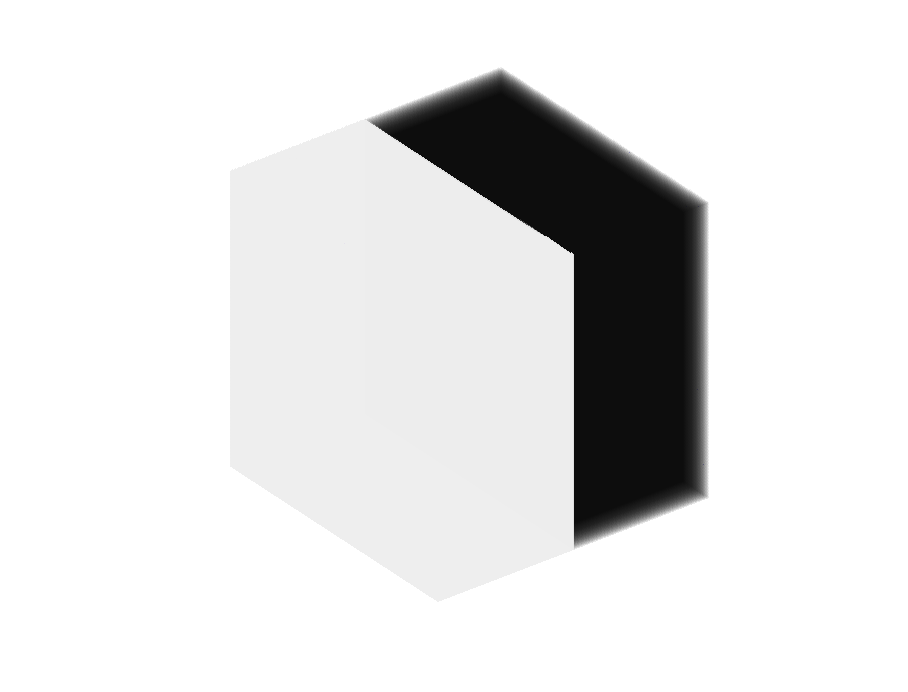
\includegraphics[scale=0.2]{intensity3d} &
					
\includegraphics[scale=0.2]{colourinterface3d}\\
					a & b\\		
					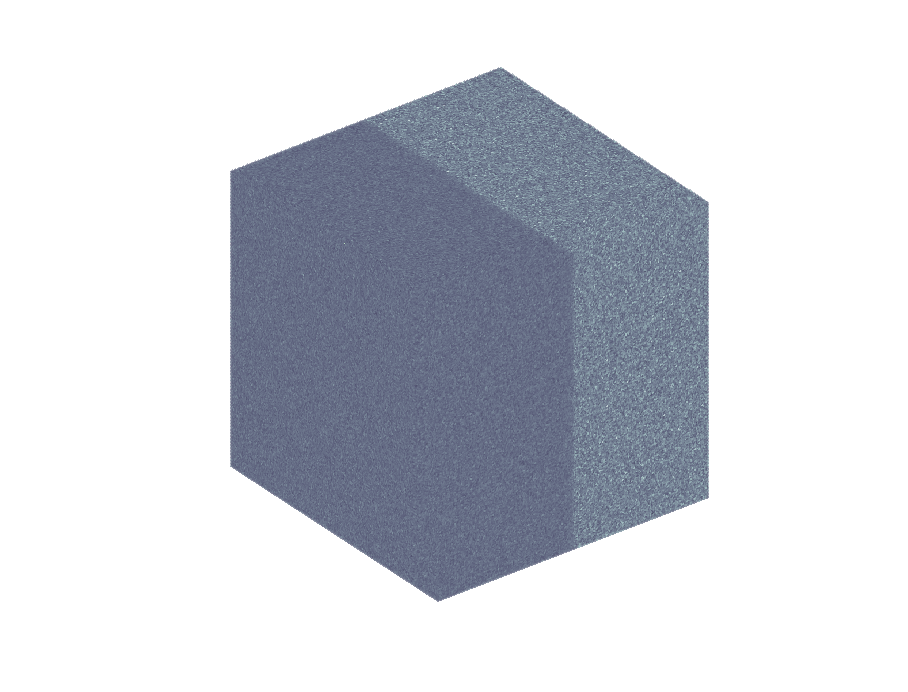
\includegraphics[scale=0.2]{statinterface} &	
					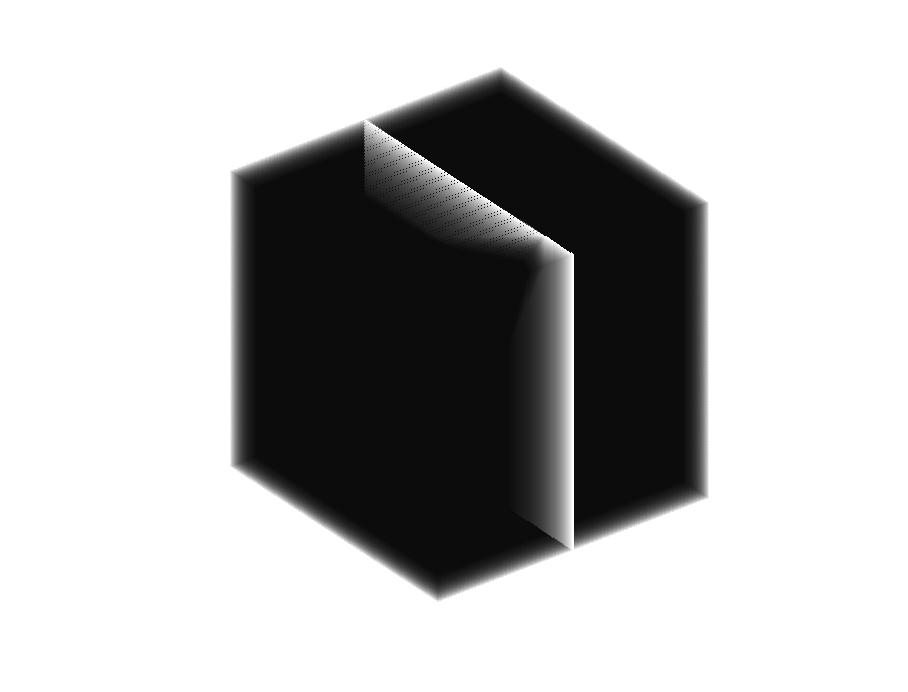
\includegraphics[scale=0.2]{edge3d2}\\
					c & d							
			\end{tabular}						
					\caption{ a) Intensity Interface. b) Colour Interface. c) Texture Interface. d) Interface Location}
			\end{figure}	
\end{frame}
%--------------------------------------------------------
\subsection{Problems}
%--------------------------------------------------------	
\begin{frame}
		\frametitle{3D Surfaces}
				\begin{itemize}
					\item Optimal plane of application is not known a priori
					\item Surfaces which lie in the plane of edge detection are not detected. Instead an outer edge of the surface is identified
				\end{itemize}
				\begin{flushright}
						\begin{figure}
									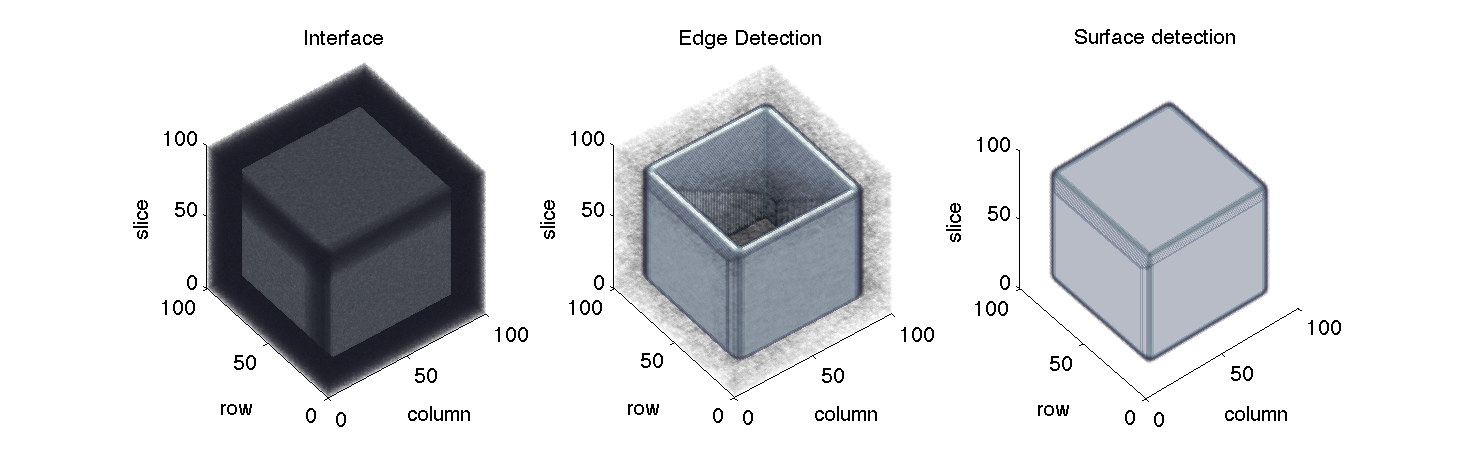
\includegraphics[scale=0.45]{fail2d}
							\end{figure}
				\end{flushright}
\end{frame}
%--------------------------------------------------------
\section{3D surface detection methods}
%--------------------------------------------------------
\begin{frame}
	\frametitle{ Criteria for edge/surface detection }
			When designing a surface detection filter, there are certain criteria that needs to be met. Canny defined the following criteria for edges, but the following holds true for surfaces.
			\begin{itemize}
				\item Criterion 1: Good detection.\\
				Minimising the number of number of missed surface points, as well as minimising the number of spurious responses.
				\item Criterion 2: Good localisation.\\
				The points marked as surface points by the operator should be as close as possible to the center of the true surface.
				\item Criterion 3: Single Response.\\
				There should be only one response to a single surface. Duplicate responses for surfaces should be eliminated.
			\end{itemize}
\end{frame}
%--------------------------------------------------------
\begin{frame}
	\frametitle{Problems}
	\begin{itemize}
	\item True 3D methods are not being utilised over multi-slice 2D methods
	\item Gradient methods fail to locate boundaries between regions of different texture when average intensity is uniform 
	\item Gradient methods require a high degree of smoothing to prevent over detection, at the expense of correct responses and accurate localisation

	\end{itemize}
\end{frame}
%--------------------------------------------------------
\begin{frame}
	\frametitle{Published Work}
	\begin{itemize}
	\item Ian Williams, Nicholas Bowring, David Svoboda, A performance evaluation of statistical tests for edge detection in textured images, Computer Vision and Image Understanding, Volume 122, May 2014, Pages 115-130,
	\item Smith, S.; Williams, I., "A Statistical Method for Improved 3D Surface Detection," in Signal Processing Letters, IEEE , vol.22, no.8, pp.1045-1049, Aug. 2015
	\end{itemize}
\end{frame}
%--------------------------------------------------------
\begin{frame}[shrink]
	\frametitle{ 2D Statistical Edge Detection}
		\begin{multicols}{2}
			\begin{itemize}
				\item Pixel intensity values are extracted using a simple 2D neighbourhood mask. 
				\item The mask is divided into two sample regions, to which a statistical test is applied measuring dissimilarity.
			 \end{itemize}
		 \begin{figure}
			\includegraphics[scale=0.35]{2D3Dmasks1}
			\caption{ Mask 1,3, not located on a boundary (low output). Mask 2 located on boundary, incorrect orientation (low output). Mask 4 located on boundary, correct orientation (high output).}
		 \end{figure}
		 \begin{itemize}
		 	\item Through a procedure of shifting the orientation of the mask, the position correlating to maximum dissimilarity then provides the output magnitude for that pixel.
		 	\item This process is repeated for each pixel in the image, evaluating the location, strength, and orientation of edges present in an image.
		 \end{itemize}
	\end{multicols}
 \end{frame}
%--------------------------------------------------------
\section{Statistical Model}
%--------------------------------------------------------
\begin{frame}
	\frametitle{Statistical Surface Detection Model}
Extending upon the two dimensional statistical edge detection method, a model for detecting surfaces can be produced.
The model should be able to:
			\begin{itemize}
					\item Detect surfaces in three dimensional image volumes.
					\item Locate interfaces that lie in the plane of the surface operator.
					\item Determine interfaces at multiple intensity scales.
					\item Be robust to noise and image artefacts. 
			\end{itemize} 
	\end{frame}
%--------------------------------------------------------
 \subsection{Maximum Response}
 %--------------------------------------------------------
 \begin{frame}
	\frametitle{ 3D Statistical Detection}
This method is a direct extension of 2D statistical edge detection into 3D.\\
	\begin{itemize}
		\item Here, voxel intensity values are extracted using a simple 3D neighbourhood mask applied across several 2D image slices. 
		\item The mask is divided into two sample regions, to which a statistical test is applied measuring dissimilarity.
	 \end{itemize}
		 \begin{figure}
		 \begin{tabular}{c c}
		 \includegraphics[scale=0.25]{2D3Dmasks1}& \includegraphics[scale=0.25]{2D3Dmasks2}
		 \end{tabular}
		 \end{figure}
	 \begin{itemize}
	 \item Through a procedure of shifting the orientation of the mask, the position correlating to maximum dissimilarity then provides the output magnitude for that voxel.
	 \item This process is repeated for each voxel in the image, evaluating the location, strength, and orientation of surfaces present in a 3D image.
	 \end{itemize}
 \end{frame}
%-------------------------------------------------------- 
\subsection{Neighbourhood Masks}
%--------------------------------------------------------
\begin{frame}
	\frametitle{Neighbourhood Mask}
		\begin{itemize}
				\item The mask neighbourhood is of equal scale in 3 dimensions
				\item To centralise the neighbourhood mask around a voxel, the mask length in each direction must be an odd value.
				\item When choosing a suitable size for a neighbourhood mask, there is a trade off between reliability and accuracy
		\end{itemize}		
	\end{frame}	
%--------------------------------------------------------
	\subsection{Mask Scale}
%--------------------------------------------------------
\begin{frame}
	\frametitle{Mask Scale}		
		\begin{block}{\textbf{As mask size increases}	}						
				\begin{itemize}
					\item Improved resolving power.
					\item Greater suppression of noise.
					\item Less susceptible to image artefacts.
					\item Image details smaller than the neighbourhood mask are not captured.
					\item More uncertainty in the location of the interface.
					\item More computationally expensive
				\end{itemize}
		\end{block}
						\textbf{Ideally we want to keep the mask as small as possible to locate finer details, while large enough to resolve texture based boundaries}				
\end{frame}
%--------------------------------------------------------
\subsection{Statistical Comparison Tests}
%--------------------------------------------------------
\begin{frame}
	\frametitle{ Statistical test }
Statistical surface detection can employ a range of different statistical comparison tests to identify different types of texture boundaries.
\begin{itemize}
\item Difference of Boxes
\item Student t-Test
\item Likelihood Test
\item Fisher Test
\item Kolmogorov-Smirnov Test
\item $\chi^{2}$ Test
\item Robust Rank Order test
\item Mann-Whitney U-Test 
\end{itemize}
\end{frame}
%--------------------------------------------------------
\begin{frame}
	\frametitle{ Student's T test }
	\begin{columns}
	\column{.40\textwidth} 	
	In probability theory, the first and second moments of a probability density function are mean and variance, therefore these two properties play a fundamental role in describing image region characteristics. The Student T test is a popular mean based statistical test which tests the hypothesis that two distributions will have a similar mean value.
	\column{.40\textwidth} 	
	\begin{block}{ $T$-test}
				\begin{equation}
					T = |\bar{x}_{A} - \bar{x}_{B}|\sqrt{\frac{N-1}{\sigma_{A}^{2} + \sigma_{B}^{2}}}
				\end{equation}
			Where $\bar{x}_{A}$, $\sigma_{A}^{2}$ and $\bar{x}_{B}$, $\sigma_{B}^{2}$ are respectively the mean and variance of mask regions A and B, and N is the number of pixels in each single region. 
			\end{block}
			\end{columns}
\end{frame}
%--------------------------------------------------------
\begin{frame}
\frametitle{ Difference of Boxes }
\begin{columns}
\column{.40\textwidth} 	
The Difference of Boxes test is the second mean based test used in this work. It's simply the absolute difference of the means of each region. This method provides similar outputs to gradient based methods.
\column{.40\textwidth} 	
\begin{block}{ Difference of Boxes -test}
			\begin{equation}
				D= |\bar{x}_{A} - \bar{x}_{B}|
			\end{equation}
		Where $\bar{x}_{A}$, and $\bar{x}_{B}$ are the mean  of mask regions A and B,. 
		\end{block}
		\end{columns}
\end{frame}
%--------------------------------------------------------
\begin{frame}
\begin{columns}
\column{.40\textwidth} 	
The $\chi^{2}$ test is a rank based test which checks for the independence of the two sorted datasets. It is a comparison measure that takes the relative difference in points at the same rank position for two binned data sets.
\column{.40\textwidth} 
\frametitle{$\chi^{2}$ Test}
\begin{block}{$\chi^{2}$ Test}

\begin{equation}
\chi^{2} = \sum_{i} \frac{R_{i}-S_{i}}{R_{i} + S_{i}}
\end{equation}
Here $R_{i}$ is the number of values in \textit{bin} $i$ of region $A$, and $S_{i}$ is the number of values in  \textit{bin} $i$ of region $B$.
\end{block}
\end{columns}
\end{frame}
%--------------------------------------------------------
\begin{frame}
	\frametitle{Two sample Kolmogorov-Smirnov test}			
				\begin{columns}
						\column{.35\textwidth} 	
					\begin{figure}
					\vspace*{-2cm}	
							\includegraphics[scale=0.7]{ks1}
					\end{figure}
Where $F_{1,n}$ and $F_{2,n}$ are the empirical distribution functions of the two samples 
						\column{.55\textwidth} 	
\begin{block}{KS-Test} 
%\vspace*{-0.5cm}	
\[  D_{n,n'} = \sup \vert F_{1,n}(x)-F_{2,n'}(y) \vert  \] 
\end{block}
					\begin{figure}
					%	\vspace*{-1cm}	
							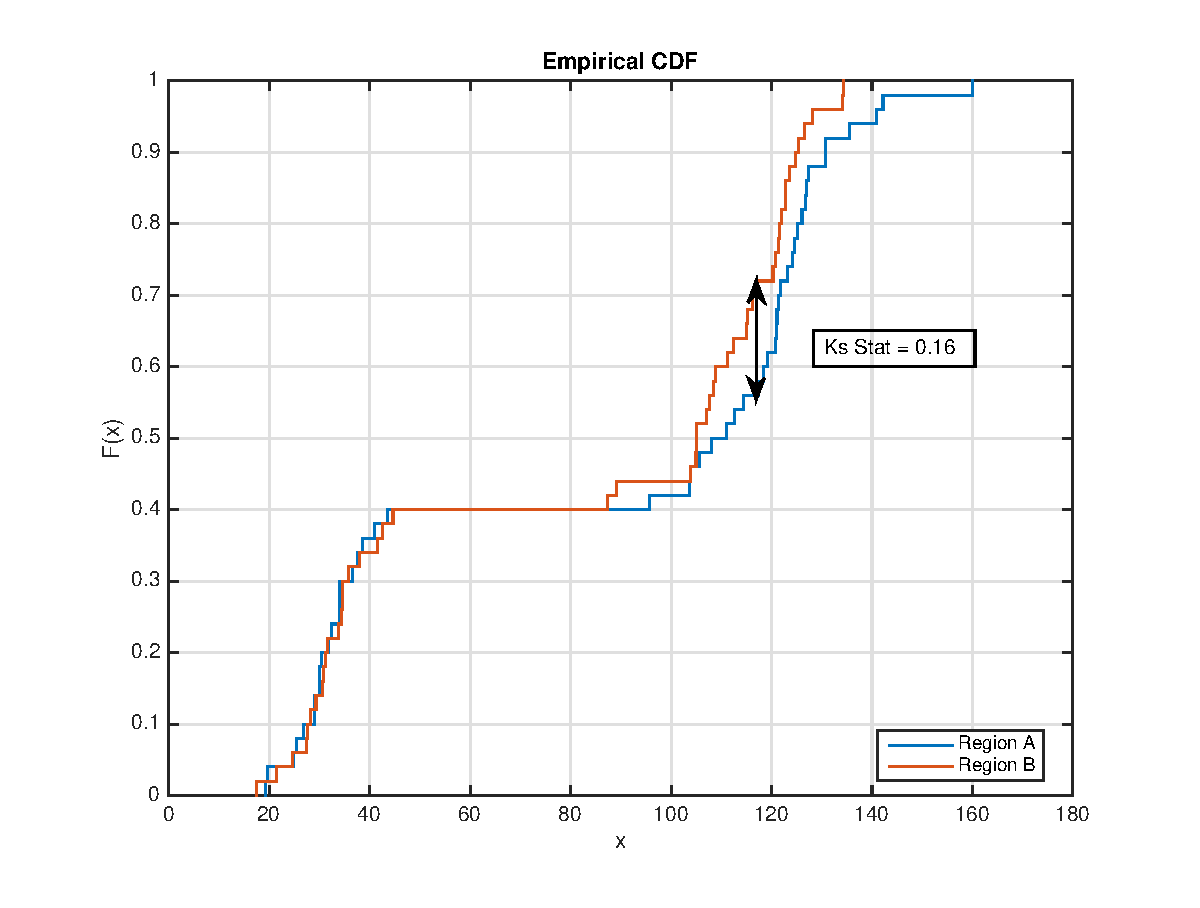
\includegraphics[scale=0.3]{cdf3.eps}
					\end{figure}
		\end{columns}
\end{frame}
%--------------------------------------------------------	
	\begin{frame}
			\frametitle{Two sample Kolmogorov-Smirnov test}				
				\begin{columns}
						\column{.35\textwidth} 	
					\begin{figure}
					\vspace*{-2cm}	
							\includegraphics[scale=0.7]{ks3}
					\end{figure}
Where $F_{1,n}$ and $F_{2,n}$ are the empirical distribution functions of the two samples 
						\column{.55\textwidth} 	
\begin{block}{KS-Test} 
%\vspace*{-0.5cm}	
\[  D_{n,n'} = \sup \vert F_{1,n}(x)-F_{2,n'}(y) \vert  \] 

\end{block}
					\begin{figure}
					%	\vspace*{-1cm}	
							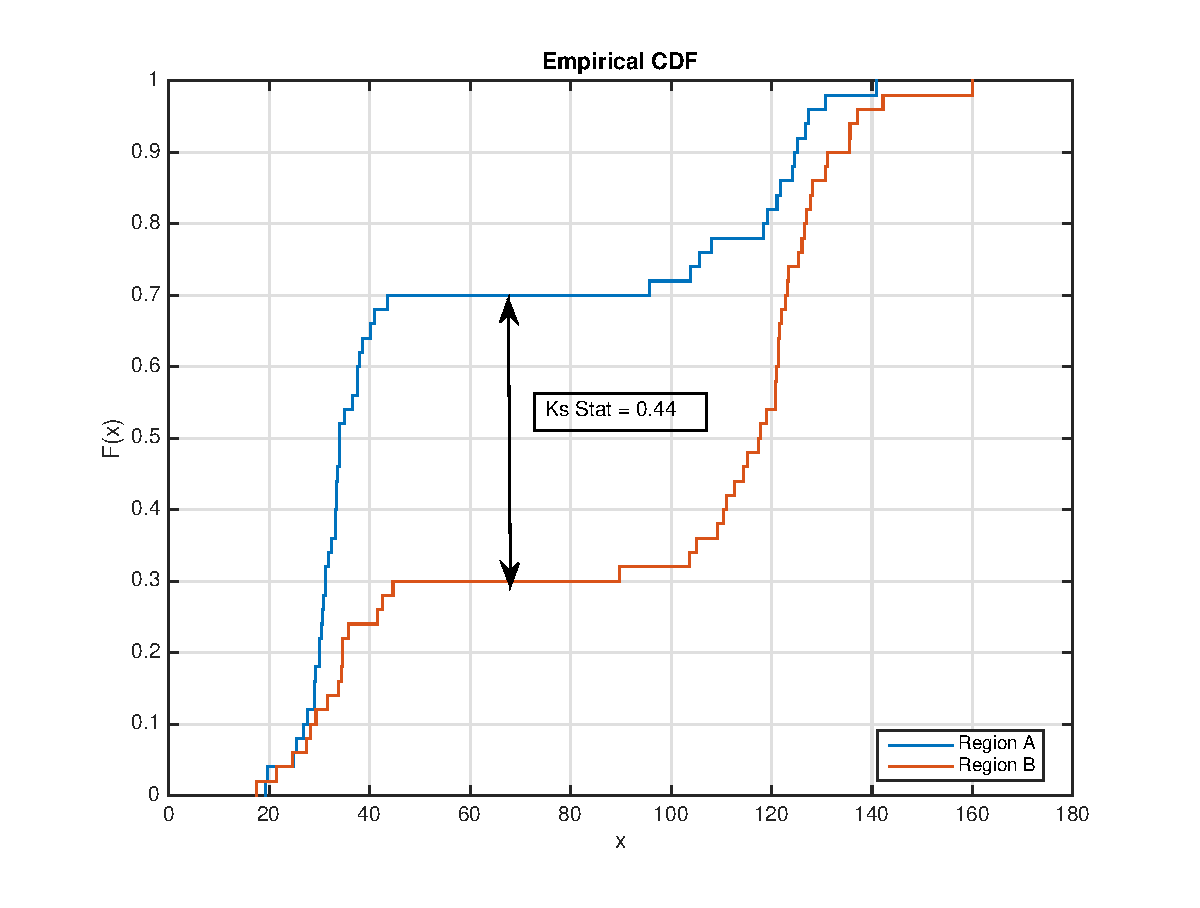
\includegraphics[scale=0.3]{cdf1.eps}
					\end{figure}
		\end{columns}
\end{frame}
%--------------------------------------------------------
	\begin{frame}
			\frametitle{Two sample Kolmogorov-Smirnov test}				
				\begin{columns}
						\column{.35\textwidth} 	
					\begin{figure}
					\vspace*{-2cm}	
							\includegraphics[scale=0.7]{ks2}
					\end{figure}
Where $F_{1,n}$ and $F_{2,n}$ are the empirical distribution functions of the two samples 
						\column{.55\textwidth} 	
\begin{block}{KS-Test} 
%\vspace*{-0.5cm}	
\[  D_{n,n'} = \sup \vert F_{1,n}(x)-F_{2,n'}(y) \vert  \] 

\end{block}
					\begin{figure}
					%	\vspace*{-1cm}	
							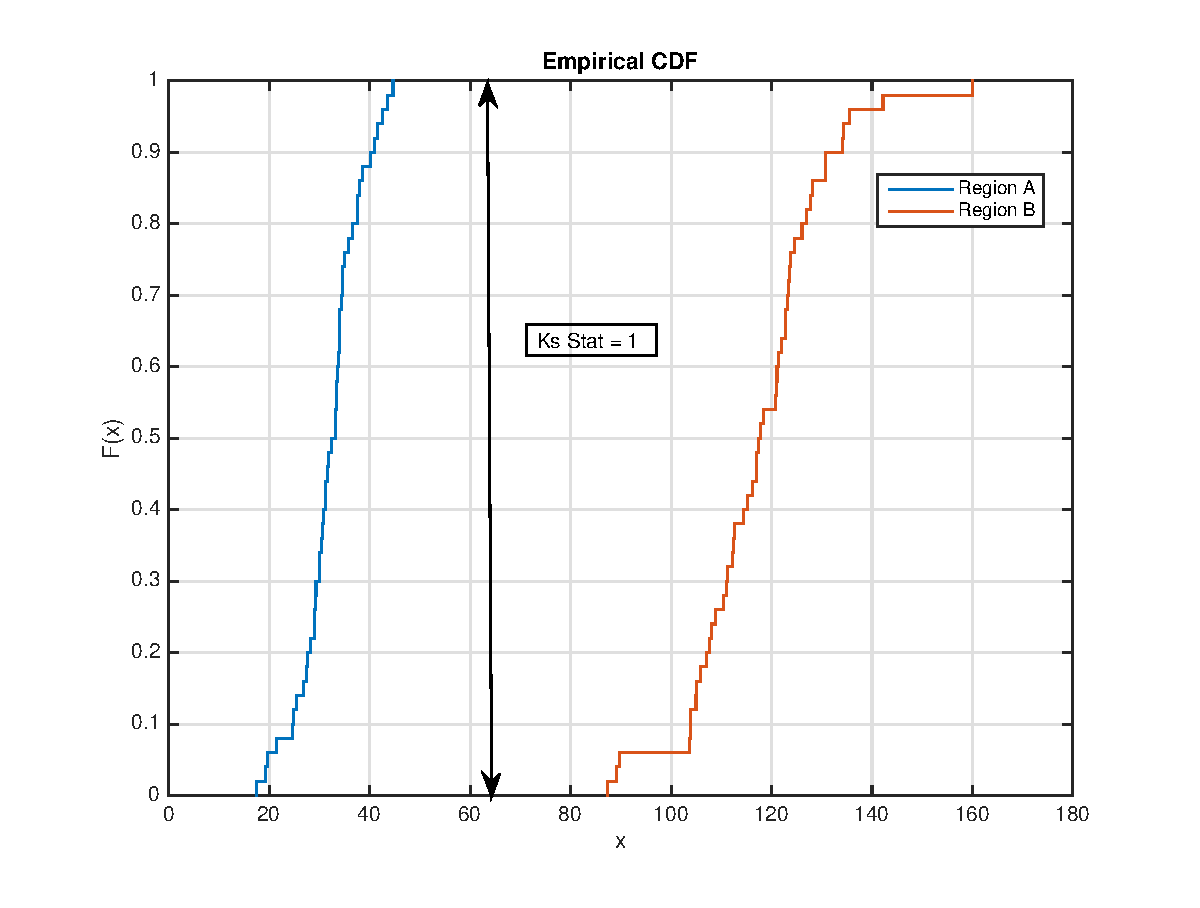
\includegraphics[scale=0.3]{cdf2.eps}
					\end{figure}
		\end{columns}
\end{frame}

\addtocontents{toc}{\newpage} % Split table in contents into second column here (requires 2 refreshes)	
\section{Methodology}
%--------------------------------------------------------
\begin{frame}
\frametitle{Matlab}
\end{frame}
%--------------------------------------------------------
	\subsection{Synthetic Data Creation}
%--------------------------------------------------------
\begin{frame}
	\frametitle{Problems}
\end{frame}
%--------------------------------------------------------
\begin{frame}
	\frametitle{Solutions}
\end{frame}
%--------------------------------------------------------
\begin{frame}
	\frametitle{Synthetic Data Creation}
	\begin{itemize}
	\item Assessing the performance of surface detection methods is non-trivial if reliant on real world image data. This is due to the fact defining a ground truth data for real imagery is near impossible, and completely dependent on the scale which which one defines the existence of a boundary.
	\item By creating synthetic images, we can accurately determine the ground truth solutions.
	\item There are numerous considerations to be made when creating synthetic image volumes
	\begin{itemize}
	\item Topology of interface 
	\item Type of interface
	\item Number of interfaces
	\item Bias of interfaces (major / minor lines)
	\item Scale
	\item Corners
	\item Data acquisition
	\end{itemize}
	\end{itemize}
	\end{frame}
	%--------------------------------------------------------
\begin{frame}
\frametitle{Synthetically Created Data - Single Scale}
\begin{columns}
\column{.45\textwidth} 	
\begin{figure}
\begin{tabular}{c c}
\includegraphics[scale=0.15]{ex2stair6_crop.eps} & \includegraphics[scale=0.135]{ex2stair6ideal.eps}

\end{tabular}
\end{figure}
\begin{figure}
\begin{tabular}{c c}
\includegraphics[scale=0.15]{ex2stair20_crop.eps} & \includegraphics[scale=0.135]{ex2stair20ideal.eps}

\end{tabular}
\end{figure}
\column{.45\textwidth} 
\begin{figure}	
\begin{tabular}{c c}
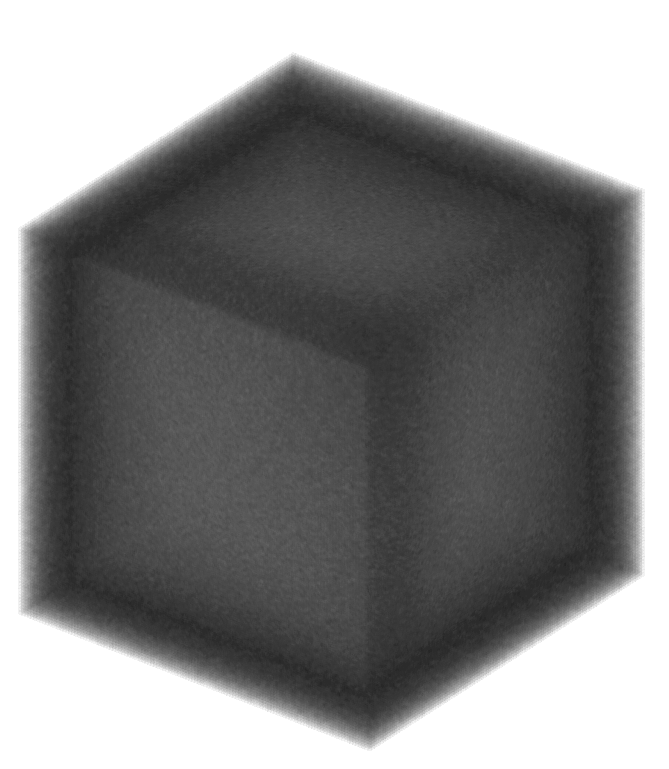
\includegraphics[scale=0.135]{cubevolume.eps}&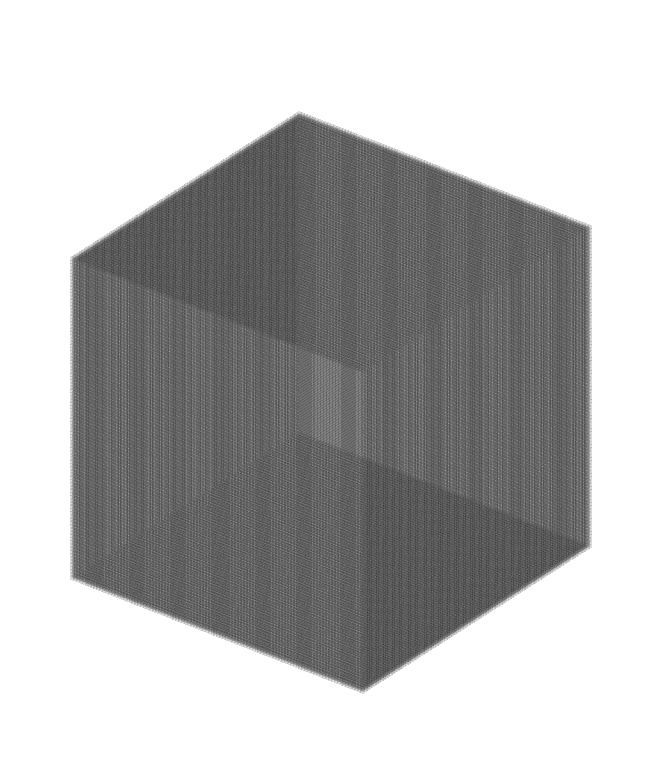
\includegraphics[scale=0.135]{cubevolumeideal.eps}
\end{tabular}
\end{figure}
\begin{figure}	
\begin{tabular}{c c}
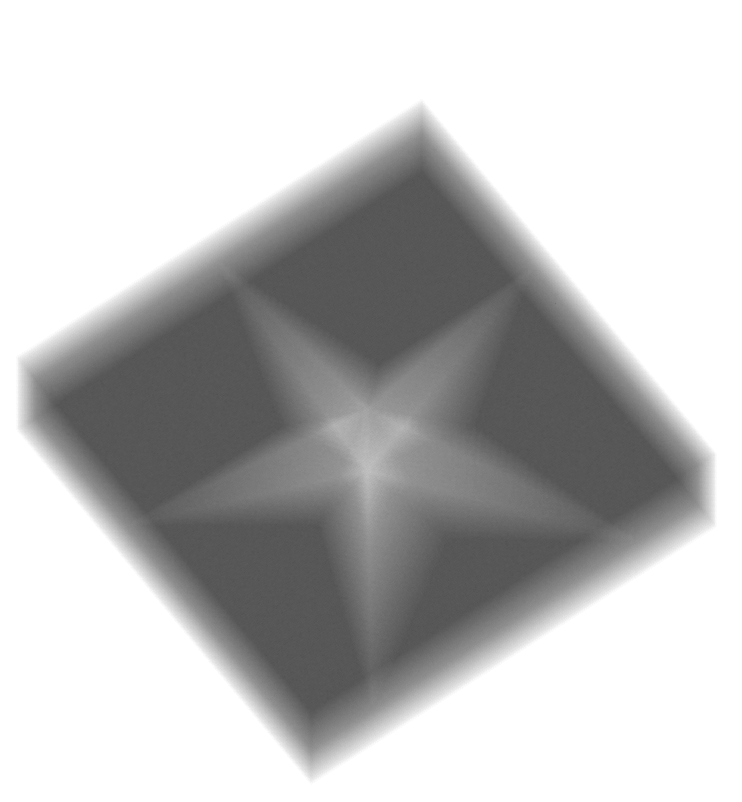
\includegraphics[scale=0.135]{star.eps}&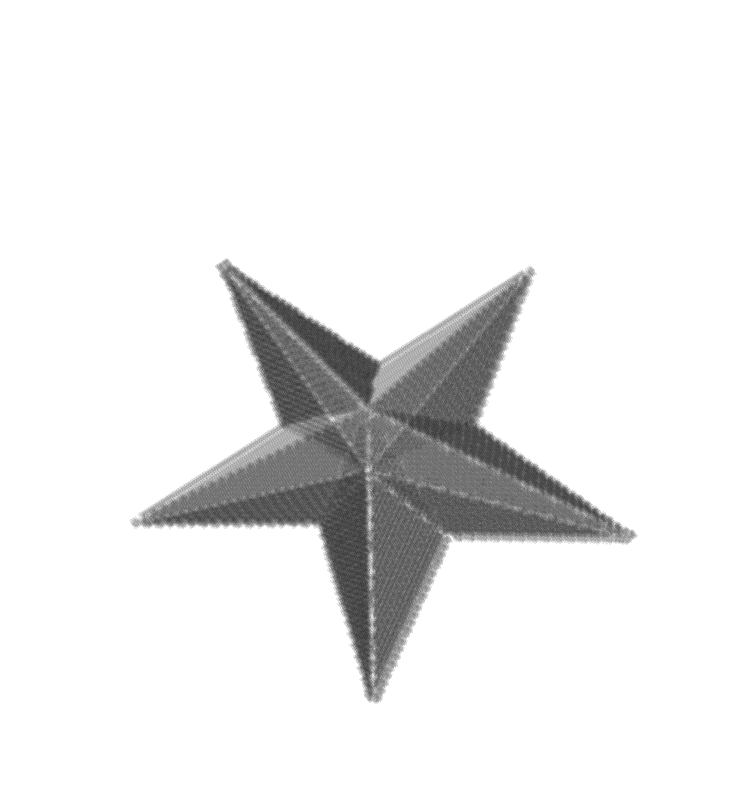
\includegraphics[scale=0.135]{starideal.eps}
\end{tabular}

\end{figure}

\end{columns}
\end{frame}	
%--------------------------------------------------------
\begin{frame}
\frametitle{Synthetically Created data - Multi Scale}
\begin{columns}
\column{.45\textwidth} 	
\begin{figure}
\begin{tabular}{cc}

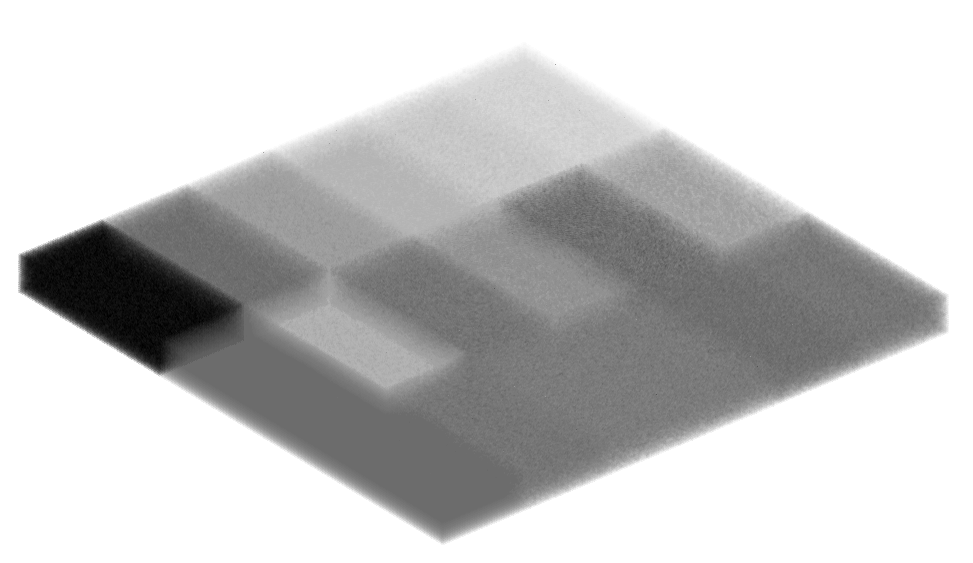
\includegraphics[scale=0.15]{multi.eps} & 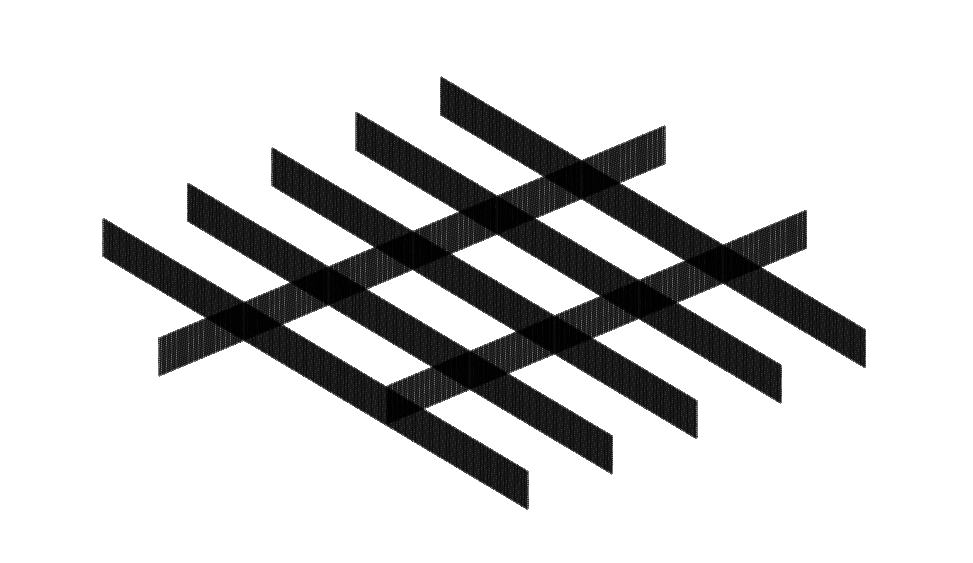
\includegraphics[scale=0.15]{multiideal.eps}

\end{tabular}
\end{figure}
\begin{figure}
\begin{tabular}{c c c}

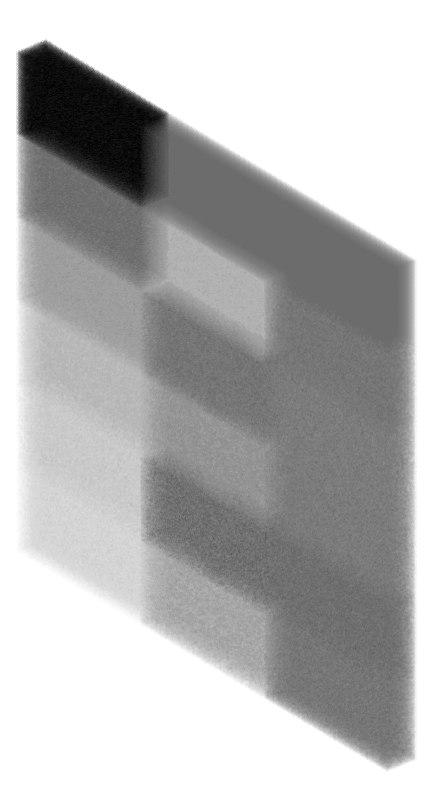
\includegraphics[scale=0.19]{multirot.eps} & &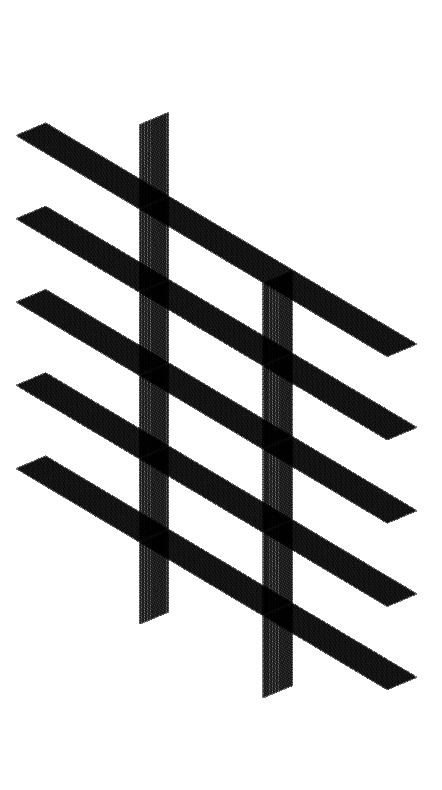
\includegraphics[scale=0.19]{multiidealrot.eps}

\end{tabular}
\end{figure}
\column{.45\textwidth} 	
\begin{figure}
\begin{tabular}{cc}

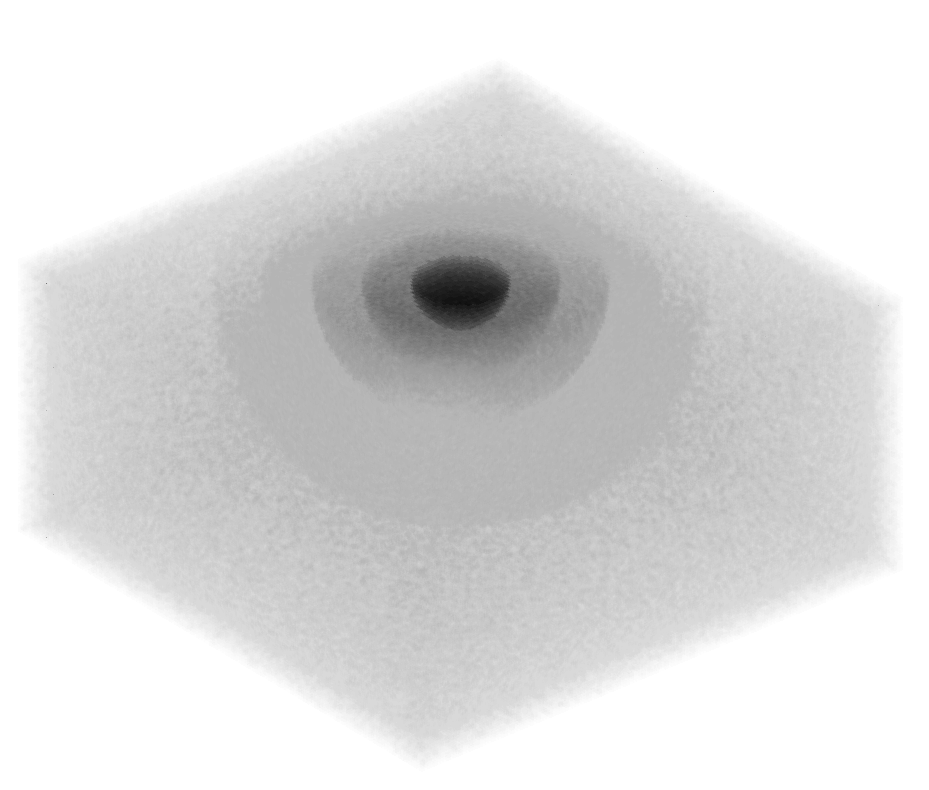
\includegraphics[scale=0.15]{sphere1.eps} & 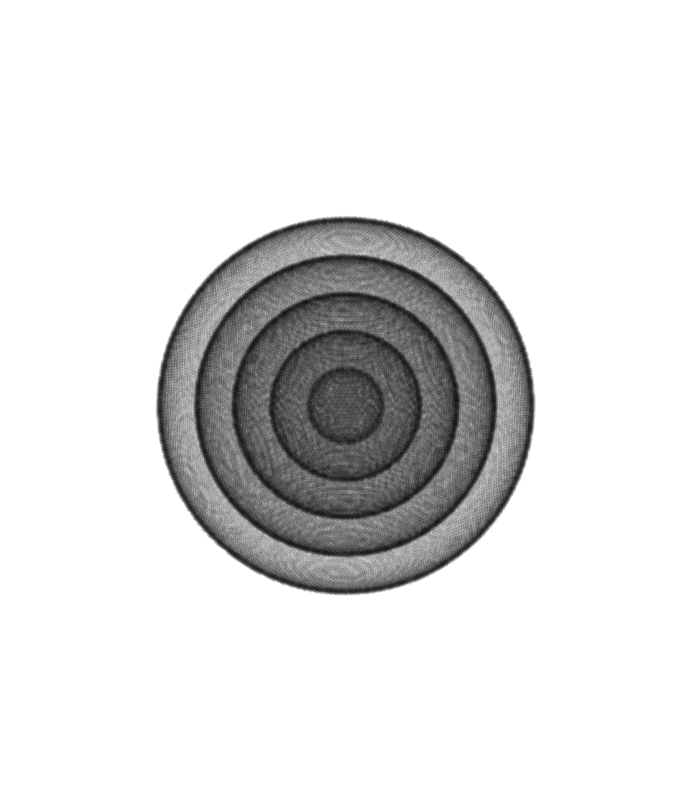
\includegraphics[scale=0.15]{sphereideal.eps}

\end{tabular}
\end{figure}
\begin{figure}
\begin{tabular}{cc}

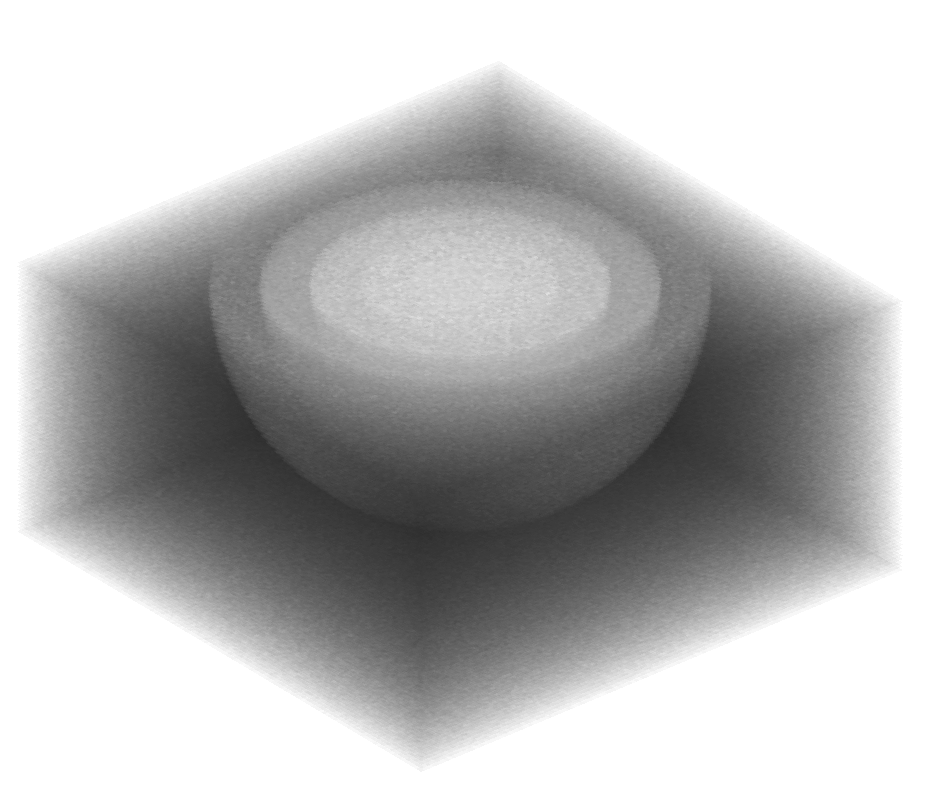
\includegraphics[scale=0.15]{sphere_reversed.eps} & 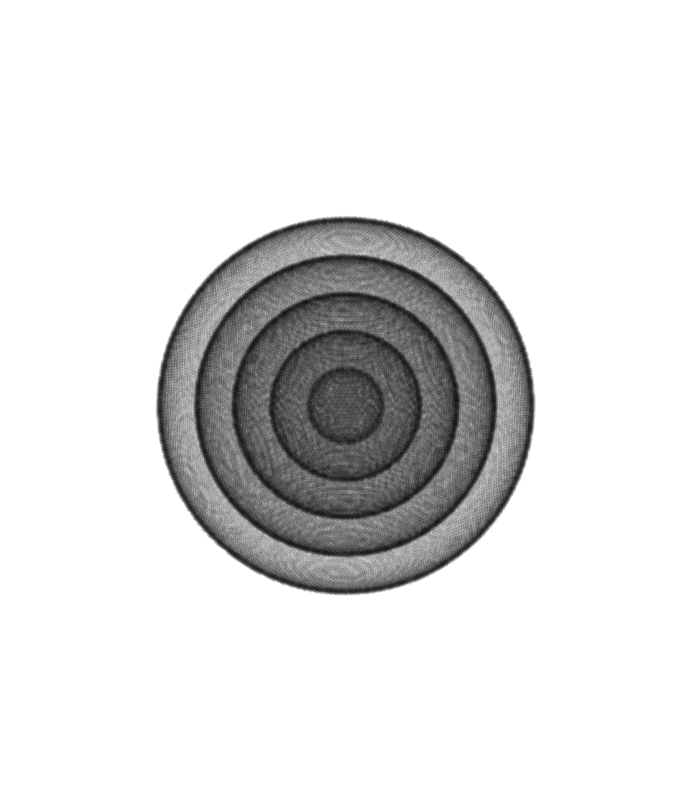
\includegraphics[scale=0.15]{sphereideal.eps}

\end{tabular}
\end{figure}
\end{columns}
\end{frame}	
%--------------------------------------------------------
\subsection{Monte Carlo Analysis}
%--------------------------------------------------------
		\begin{frame}
				\frametitle{Monte Carlo Analysis}
			 			In this study we used a Monte Carlo Methodology of testing.
			 			\begin{itemize}
			 			\item Three examples of each image
			 			\item Pseudo-random values containing the same statistical properties for each image 
			 			\item Mean and standard deviation of results of each image type determines the score.
			 			\end{itemize}
	\end{frame}
%--------------------------------------------------------
\section{Results}
\subsection{PFOM scores}
%--------------------------------------------------------
		\begin{frame}
			\frametitle{Results}
			\begin{figure}
\begin{tabular}{c c}
\includegraphics[width=0.49\textwidth]{PFOMmulti.eps}&\includegraphics[width=0.49\textwidth]{PFOMsphere.eps}
\end{tabular}
\end{figure}
	\end{frame}
			\begin{frame}
			\frametitle{Results}
			\begin{figure}
\begin{tabular}{c c}
\includegraphics[width=0.49\textwidth]{ROC1.eps}&\includegraphics[width=0.49\textwidth]{PR1.eps}
\end{tabular}
\end{figure}
	\end{frame}
	%--------------------------------------------------------
\subsection{Visual Results}
\subsubsection{Sphere}
%--------------------------------------------------------
\begin{frame}

\frametitle{Visual Results - Sphere}
\begin{columns}
\column{.2\textwidth}
\vspace{-2cm}
\begin{figure}
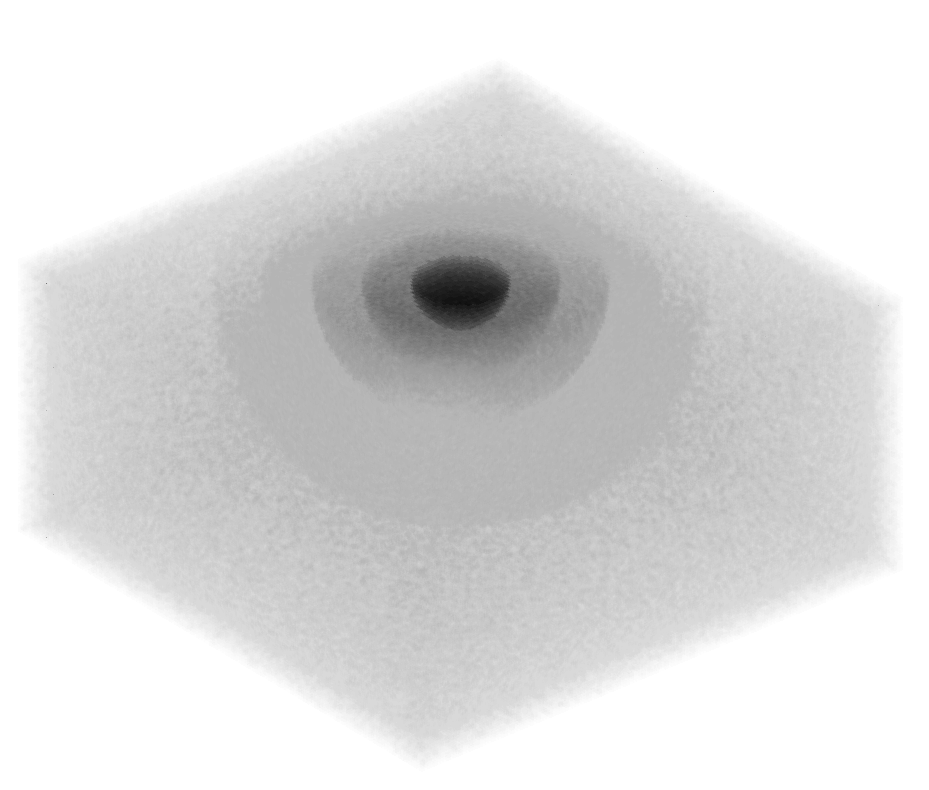
\includegraphics[width=1\textwidth]{sphere1.eps}
\end{figure}
\column{.60\textwidth}  
\begin{figure}
\begin{tabular}{c c c }
%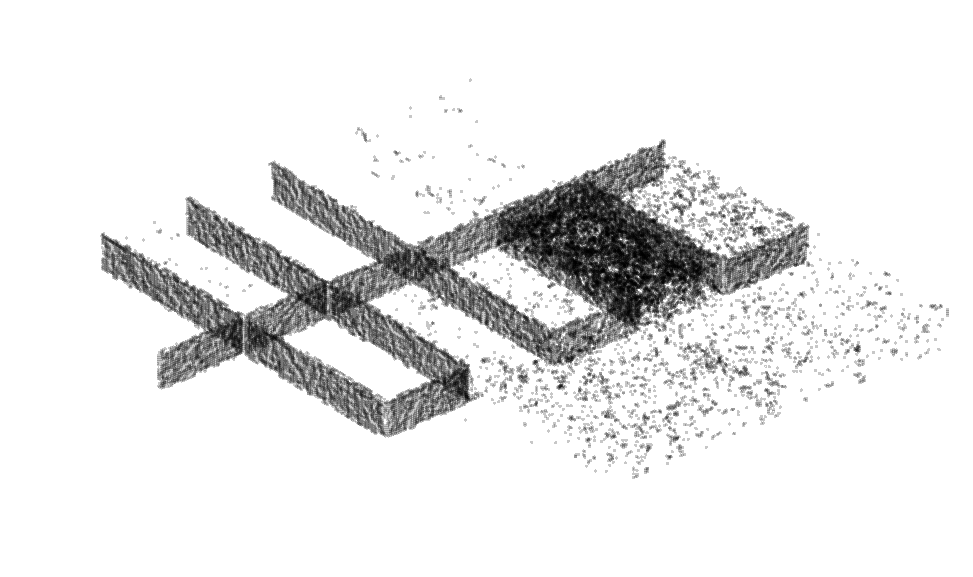
\includegraphics[scale=0.2]{Cannysigma3}&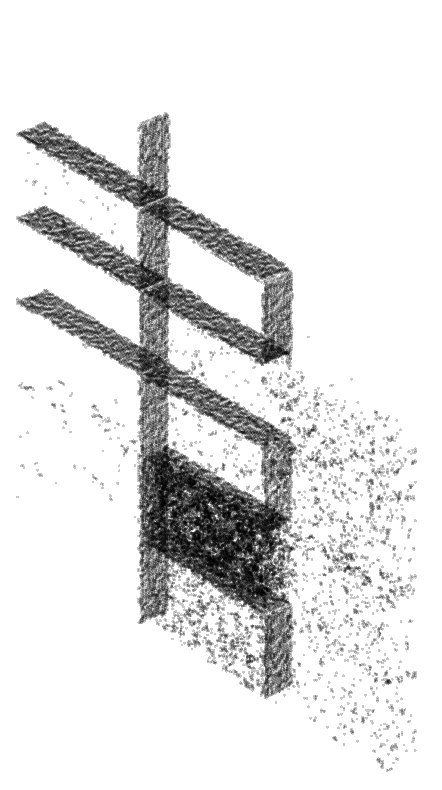
\includegraphics[scale=0.2]{Cannysigma3rot}&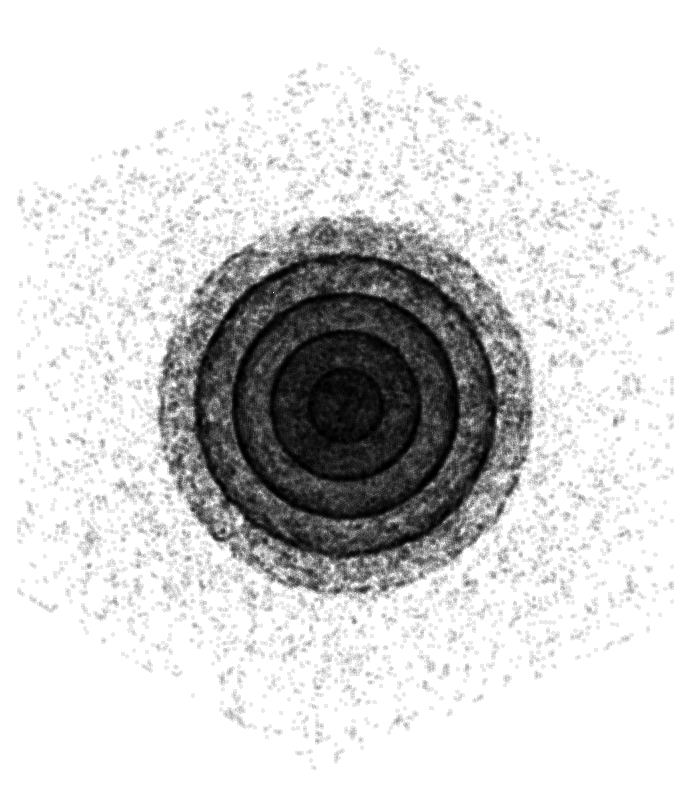
\includegraphics[scale=0.2]{Cannysigma3sphere}&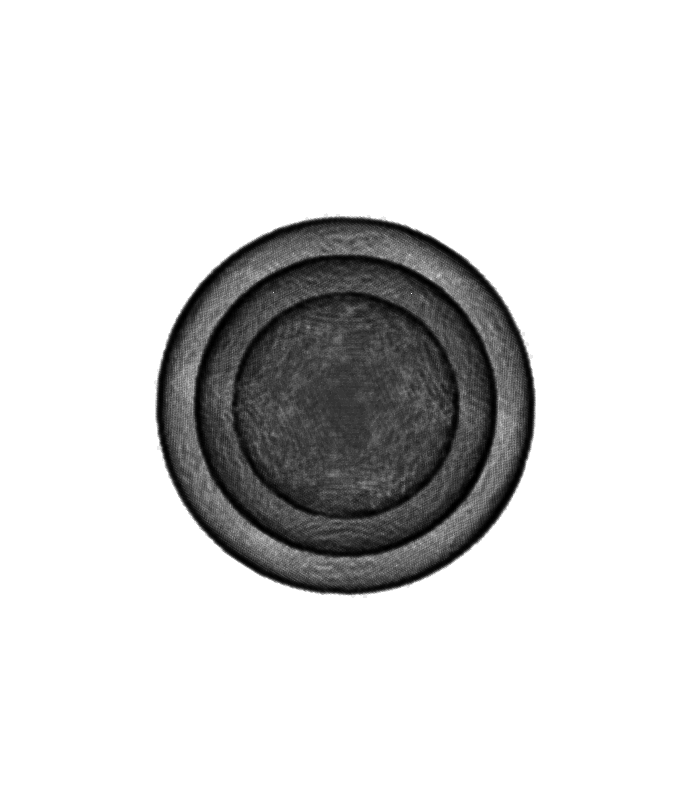
\includegraphics[scale=0.2]{Cannysigma3sphereR}\\
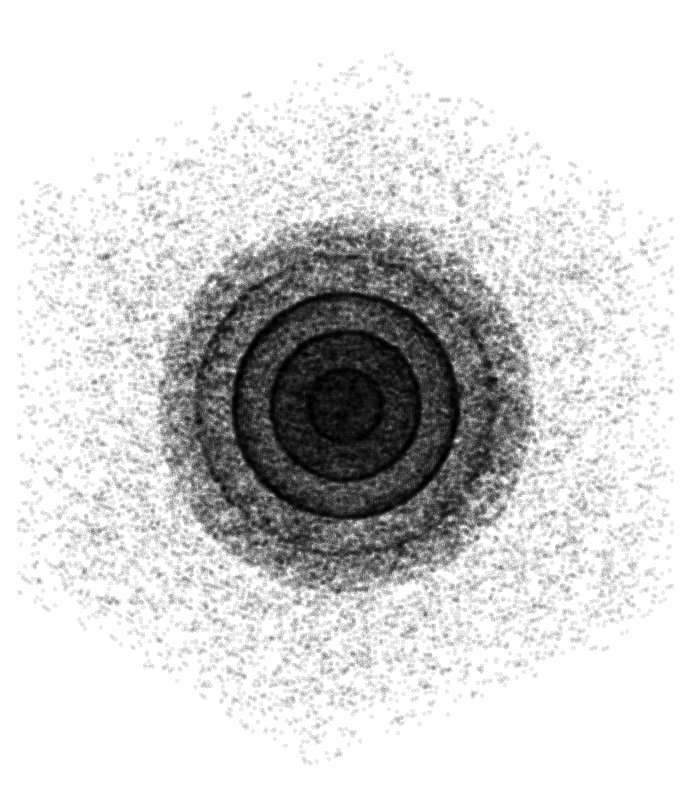
\includegraphics[scale=0.18]{canny2dsphere.eps}&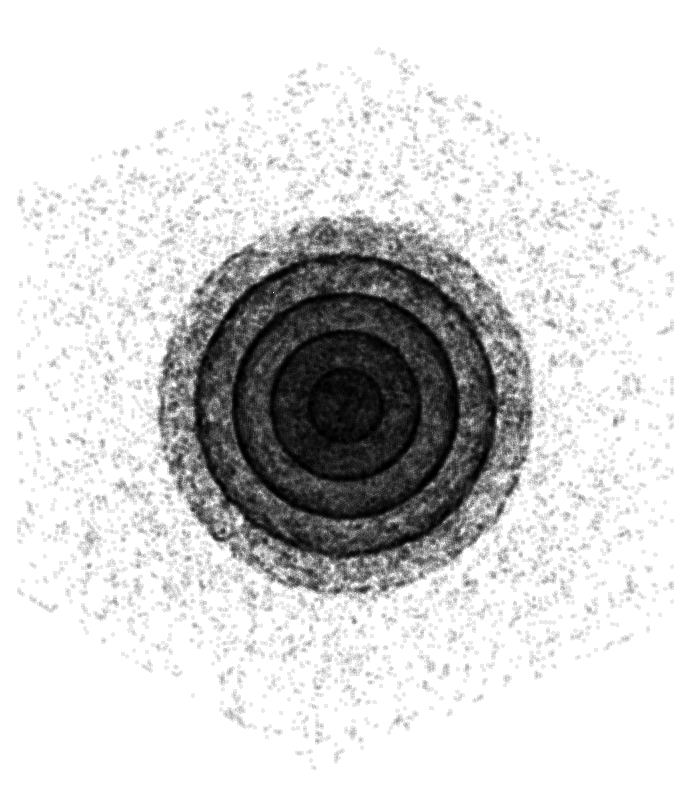
\includegraphics[scale=0.18]{Cannysigma3sphere}&\includegraphics[scale=0.18]{SteerableFilterSigma2sphere}\\
a & b & c \\
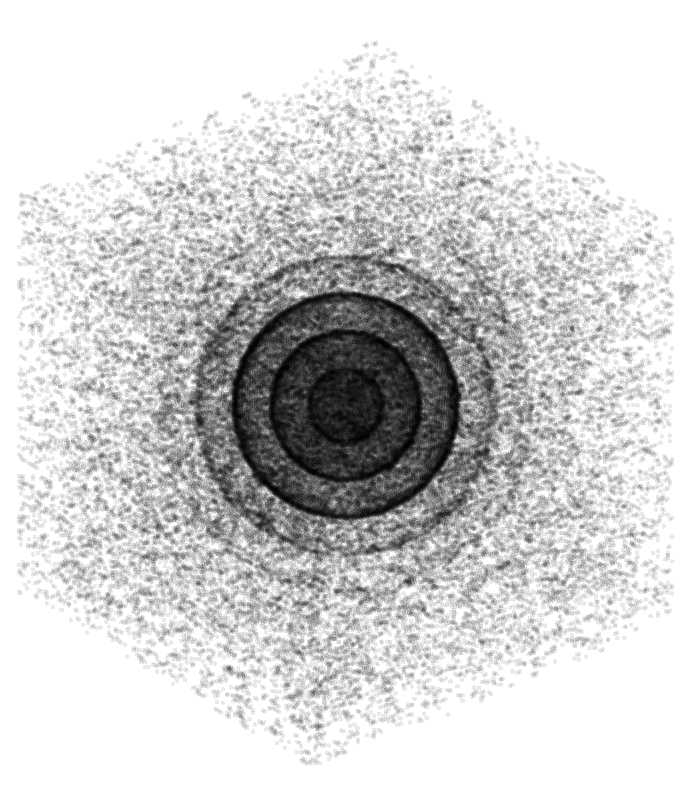
\includegraphics[scale=0.18]{stat2dsphere.eps}& 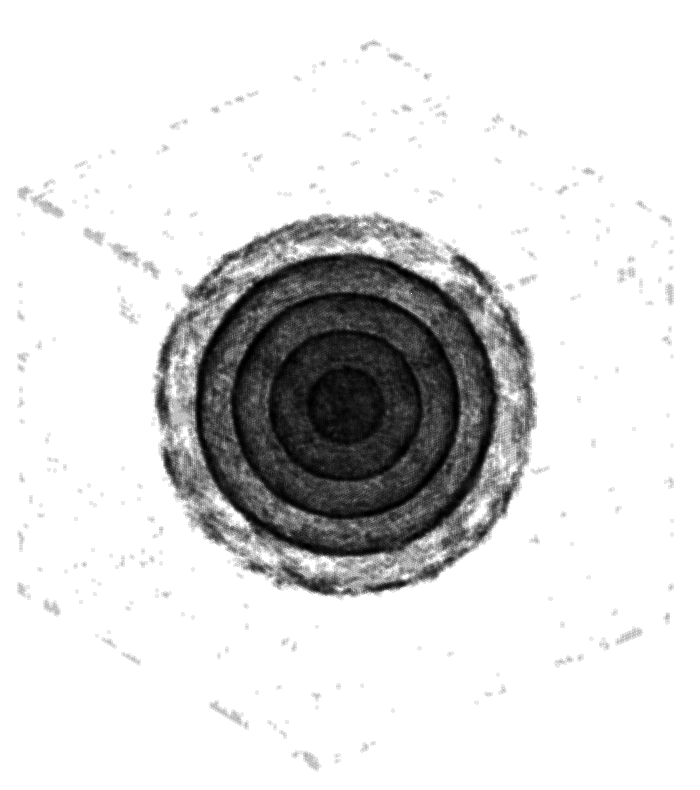
\includegraphics[scale=0.18]{T3_sphere}&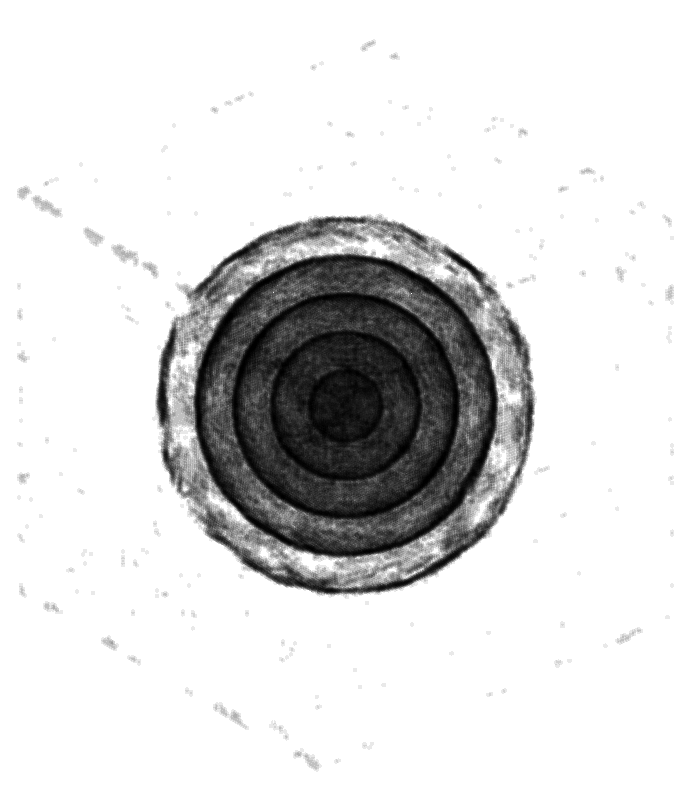
\includegraphics[scale=0.18]{T13_sphere}\\

d & e & f\\

\end{tabular}
\caption{ a) Canny 2D. b) Canny 3D. c) Steerable. d) 2D Statistical. e) 3D Statistical  f) 3D Statistical.}
\end{figure}
\column{.2\textwidth} 
\vspace{-2cm}
\begin{figure}
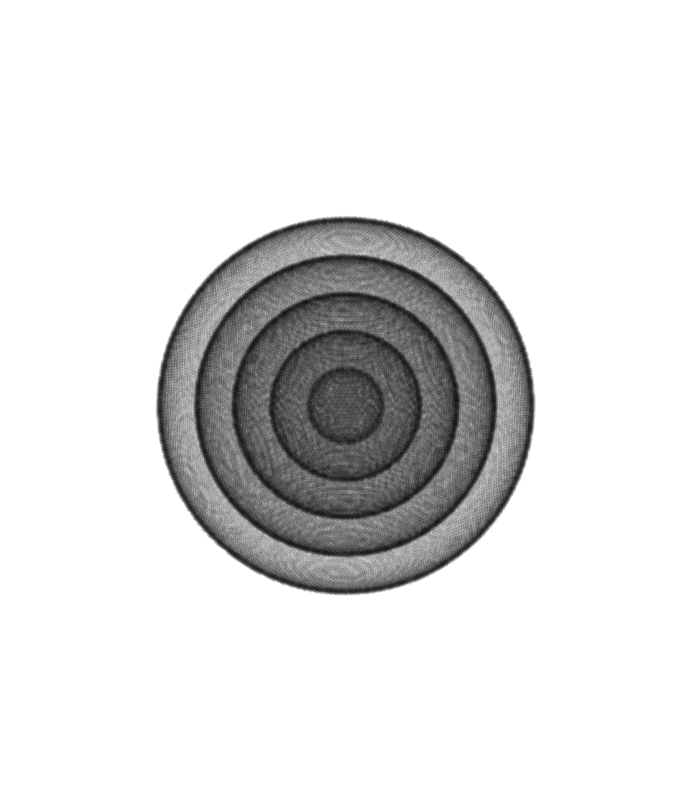
\includegraphics[width=1\textwidth]{sphereideal.eps}
\end{figure}
\end{columns}
\end{frame}
%--------------------------------------------------------
\subsubsection{Sphere Reversed}
%--------------------------------------------------------
\begin{frame}

\frametitle{Visual Results -Sphere Reversed}
\begin{columns}
\column{.2\textwidth}
\vspace{-2cm}
\begin{figure}
\includegraphics[width=1\textwidth]{sphere_reversed.eps}
\end{figure}
\column{.60\textwidth}  
\begin{figure}
\begin{tabular}{c c c }
%\includegraphics[scale=0.2]{SteerableFilterSigma2}&\includegraphics[scale=0.2]{SteerableFilterSigma2rot}&\includegraphics[scale=0.2]{SteerableFilterSigma2sphere}&\includegraphics[scale=0.2]{SteerableFilterSigma2sphereR}\\
\includegraphics[scale=0.18]{canny2dsphereR.eps}&\includegraphics[scale=0.18]{Cannysigma3sphereR}&\includegraphics[scale=0.18]{SteerableFilterSigma2sphereR}\\
a & b & c\\
\includegraphics[scale=0.18]{stat2dsphereR.eps} & \includegraphics[scale=0.18]{T3_sphereR}&\includegraphics[scale=0.18]{T13_sphereR}\\

d & e & f\\
\end{tabular}
\caption{ a) Canny 2D. b) Canny 3D. c) Steerable. d) 2D Statistical. e) 3D Statistical  f) 3D Statistical.}
\end{figure}
\column{.2\textwidth}
\vspace{-2cm}
\begin{figure}
\includegraphics[width=1\textwidth]{sphereideal.eps}
\end{figure}
\end{columns}
\end{frame}
%--------------------------------------------------------
\subsubsection{Multiple Scale}
%--------------------------------------------------------
\begin{frame}[shrink]
\frametitle{Visual Results - Multiple Scale}
\begin{columns}
\column{.2\textwidth}
\vspace{-2cm}
\begin{figure}
\includegraphics[width=0.9\textwidth]{multi.eps}
\end{figure}
\column{.60\textwidth}  
\begin{figure}
\begin{tabular}{c c c }
%\includegraphics[scale=0.2]{T3_11}&\includegraphics[scale=0.2]{T3_9}&\includegraphics[scale=0.2]{T3_sphere}&\includegraphics[scale=0.2]{T3_sphereR}\\
\includegraphics[width=0.30\textwidth]{canny2dmulti}&\includegraphics[width=0.30\textwidth]{Cannysigma3}&\includegraphics[width=0.30\textwidth]{SteerableFilterSigma2}\\
a & b & c \\
\includegraphics[width=0.30\textwidth]{stat2dmulti.eps}&\includegraphics[width=0.30\textwidth]{T3_11}&\includegraphics[width=0.30\textwidth]{T13_9}\\
d & e & f\\

\end{tabular}
\caption{ a) Canny 2D. b) Canny 3D. c) Steerable. d) 2D Statistical. e) 3D Statistical  f) 3D Statistical.}
\end{figure}
\column{.2\textwidth}
\vspace{-2cm}
\begin{figure}
\includegraphics[width=0.9\textwidth]{multiideal.eps}
\end{figure}
\end{columns}
\end{frame}
%--------------------------------------------------------
\subsubsection{Multiple Scale Rotated}
%--------------------------------------------------------
\begin{frame}
\frametitle{Visual Results - Multiple Scale Rotated}
\begin{columns}
\column{.2\textwidth}
\vspace{-2cm}
\begin{figure}
\includegraphics[width=0.6\textwidth]{multirot.eps}
\end{figure}
\column{.60\textwidth}  
\begin{figure}
\begin{tabular}{c c  c }
%\includegraphics[scale=0.2]{T13_9}&\includegraphics[scale=0.2]{T13_9rot}&\includegraphics[scale=0.2]{T13_sphere}&\includegraphics[scale=0.2]{T13_sphereR}\\
\includegraphics[width=0.20\textwidth]{canny2dmultiR}&\includegraphics[width=0.20\textwidth]{Cannysigma3rot}&\includegraphics[width=0.20\textwidth]{SteerableFilterSigma2rot}\\
a & b & c \\
\includegraphics[width=0.20\textwidth]{stat2dmultiR.eps}&\includegraphics[width=0.20\textwidth]{T3_9}&\includegraphics[width=0.20\textwidth]{T13_9rot}\\
d & e & f\\

\end{tabular}
\caption{ a) Canny 2D. b) Canny 3D. c) Steerable. d) 2D Statistical. e) 3D Statistical  f) 3D Statistical.}
\end{figure}
\column{.2\textwidth}
\vspace{-2cm}
\begin{figure}
\includegraphics[width=0.6\textwidth]{multiidealrot.eps}
\end{figure}
\end{columns}
\end{frame}
%--------------------------------------------------------
\subsection{MRI Results}
%--------------------------------------------------------
\begin{frame}
\frametitle{Real Image Results}
\begin{figure}
\begin{tabular}{c c c}
\includegraphics[scale=0.25]{headsteer}&\includegraphics[scale=0.25]{headcanny}&\includegraphics[scale=0.25]{headT}\\
Steerable & Canny & Statistical

\end{tabular}
\end{figure}
\end{frame}
%--------------------------------------------------------
\section{Conclusions}
\subsection{Conclusions}
%--------------------------------------------------------
\begin{frame}
\frametitle{Conclusions}
\begin{itemize}
\item Outperforms 3D Canny and Steerable filters, improved response to texture and noise.
\item Outperforms all 2D edge detection methods.
\item When possible, 3D surface detection should always be used instead of 2D, and where texture defines image boundaries, Statistical methods should be employed.
\end{itemize}
 
\end{frame}
%--------------------------------------------------------
\subsection{Future Work}
%--------------------------------------------------------
\begin{frame}
\frametitle{ Future Work }
\begin{itemize}
\item Synthetic data creation.
\item Statistical tests
\item Mask shape
\item Real World application testing. (Active Contours/surfaces, snakes GVFCs, etc) 
\end{itemize}
\end{frame}
%--------------------------------------------------------
\subsection{End}


%--------------------------------------------------------
	
	\end{document}
